\documentclass{exam}

\usepackage{units} 
\usepackage[fleqn]{amsmath}
\usepackage{float}
\usepackage{mdwlist}
\usepackage{booktabs}
\usepackage{caption}
\usepackage{fullpage}
\usepackage{enumerate}
\usepackage{graphicx}

\usepackage{2in1, lscape} 

\everymath{\displaystyle}

\printanswers

\title{Statistics \\ Week Four}
\date{\today}
\author{}

\begin{document}

\maketitle
\tableofcontents

  \section{Homework}

  \begin{itemize*}
    \item TO DO
  \end{itemize*}

  \section{Regression}

  \begin{figure}[H]
    \centering
    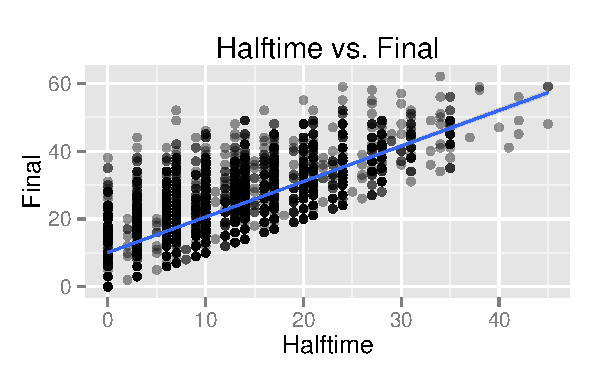
\includegraphics{figures/nfl/ht_vs_final.pdf}
    \caption{Halftime vs. Final Score}
  \end{figure}

  \begin{figure}[H]
    \centering
    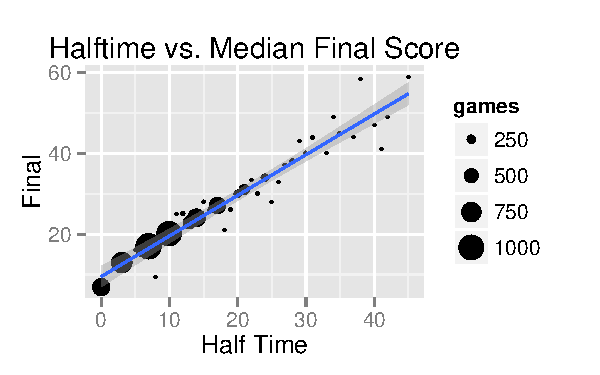
\includegraphics{figures/nfl/ht_vs_median_final.pdf}
    \caption{Halftime vs. Median Final Score}
  \end{figure}

\end{document}

